\documentclass[11pt,letterpaper]{article}
\usepackage{fullpage}
\usepackage[top=0.5in, bottom=1.5in, left=1in, right=1in]{geometry}
\usepackage{amsmath,amsthm,amsfonts,amssymb,amscd}
\usepackage{lastpage}
\usepackage{enumerate}
\usepackage{enumitem}
\usepackage{fancyhdr}
\usepackage{graphicx}
\usepackage{listings}
\usepackage{hyperref}
\usepackage{booktabs}
\usepackage{cancel}
\usepackage{physics}
\usepackage{caption,cleveref,colortbl,csquotes,datatool,helvet,mathpazo,multirow,listings,pgfplots,xcolor}

\hypersetup{%
  colorlinks=true,
  linkcolor=blue,
  linkbordercolor={0 0 1}
}

\setlength{\parindent}{0.0in}
\setlength{\parskip}{0.05in}
\setlength{\footnotesep}{1.2\baselineskip}


% edit these
\newcommand\course{AST222H}
\newcommand\Title{Problem Set 5}
\newcommand\Name{Jeff Shen} 
\newcommand\Id{1004911526} 
\newcommand\Date{3 Apr 2020}

\pagestyle{fancyplain}
\headheight 35pt
\lhead{\Name}
\lhead{\Name\\\Id}
\chead{\LARGE \Title}
\rhead{\course \\ \Date}
\lfoot{}
\cfoot{}
\rfoot{\small\thepage}
\pgfplotsset{compat=1.16}
\headsep 1.2em

\begin{document}

\section*{Problem 1}

Using the distance modulus formula, this distance is (ignoring extinction)
\begin{align*}
    d = 10^{(m-M+5)/5} = 10^{(25+19.5+5)/5} = 7.94~{\rm Gpc}.
\end{align*}

\section*{Problem 2}
Density for matter is given by $\rho_{m,\,0} = \Omega_{m,\,0}(1+z)^3$, and for radiation by $\rho_{r,\,0} = \Omega_{r,\,0}(1+z)^4$. Equate the two and solve for $z$:
\begin{alignat*}{2}
    &&\rho_{m,\,0} &= \rho_{r,\,0} \\
    \implies&&\Omega_{m,\,0}(1+z)^3 &= \Omega_{r,\,0}(1+z)^4 \\
    \implies&&z &= \frac{\Omega_{m,\,0}}{\Omega_{r,\,0}} - 1 = \frac{0.317}{10^{-4}} - 1 = 3169.
\end{alignat*}

\section*{Problem 3}

The Schwarzchild radius of the black hole is 
\begin{align*}
    R_S = \frac{2GM}{c^2} = \frac{2\times 6.67\times 10^{-11}~{\rm m^3\,kg^{-1}}\times 2\times 10^{9}~{\rm M_\odot}}{(2.99\times 10^{8}~{\rm m\,s^{-1}})^2} = 5.91\times 10^{12}~{\rm m}.
\end{align*}
Given that the distance to M87 is $53.5~{\rm Mly\footnote{from Google}} = 5.06\times 10^{23}~{\rm m}$, the angular radius is 
\begin{align*}
    \theta \simeq \tan{\theta} = \frac{R_S}{d} = \frac{5.91\times 10^{12}~{\rm m}}{5.06\times 10^{23}~{\rm m}} = 1.17\times 10^{-11}~{\rm rad} = 2.41\times 10^{-6}~{\rm arcsec}.
\end{align*}

{\huge velocity dispersion aprt? observable? something about not being observable because seeing limits the resolution of ground telescopes. velocity dispersion has something to do with full width half maximum which relates to the seeing resolution.}

\section*{Problem 4}

what? if the parallax error is the same as the distance error then isnt the distance error just 
\newpage

\section*{Problem 5}

\begin{figure*}[!htbp]
    \centering
    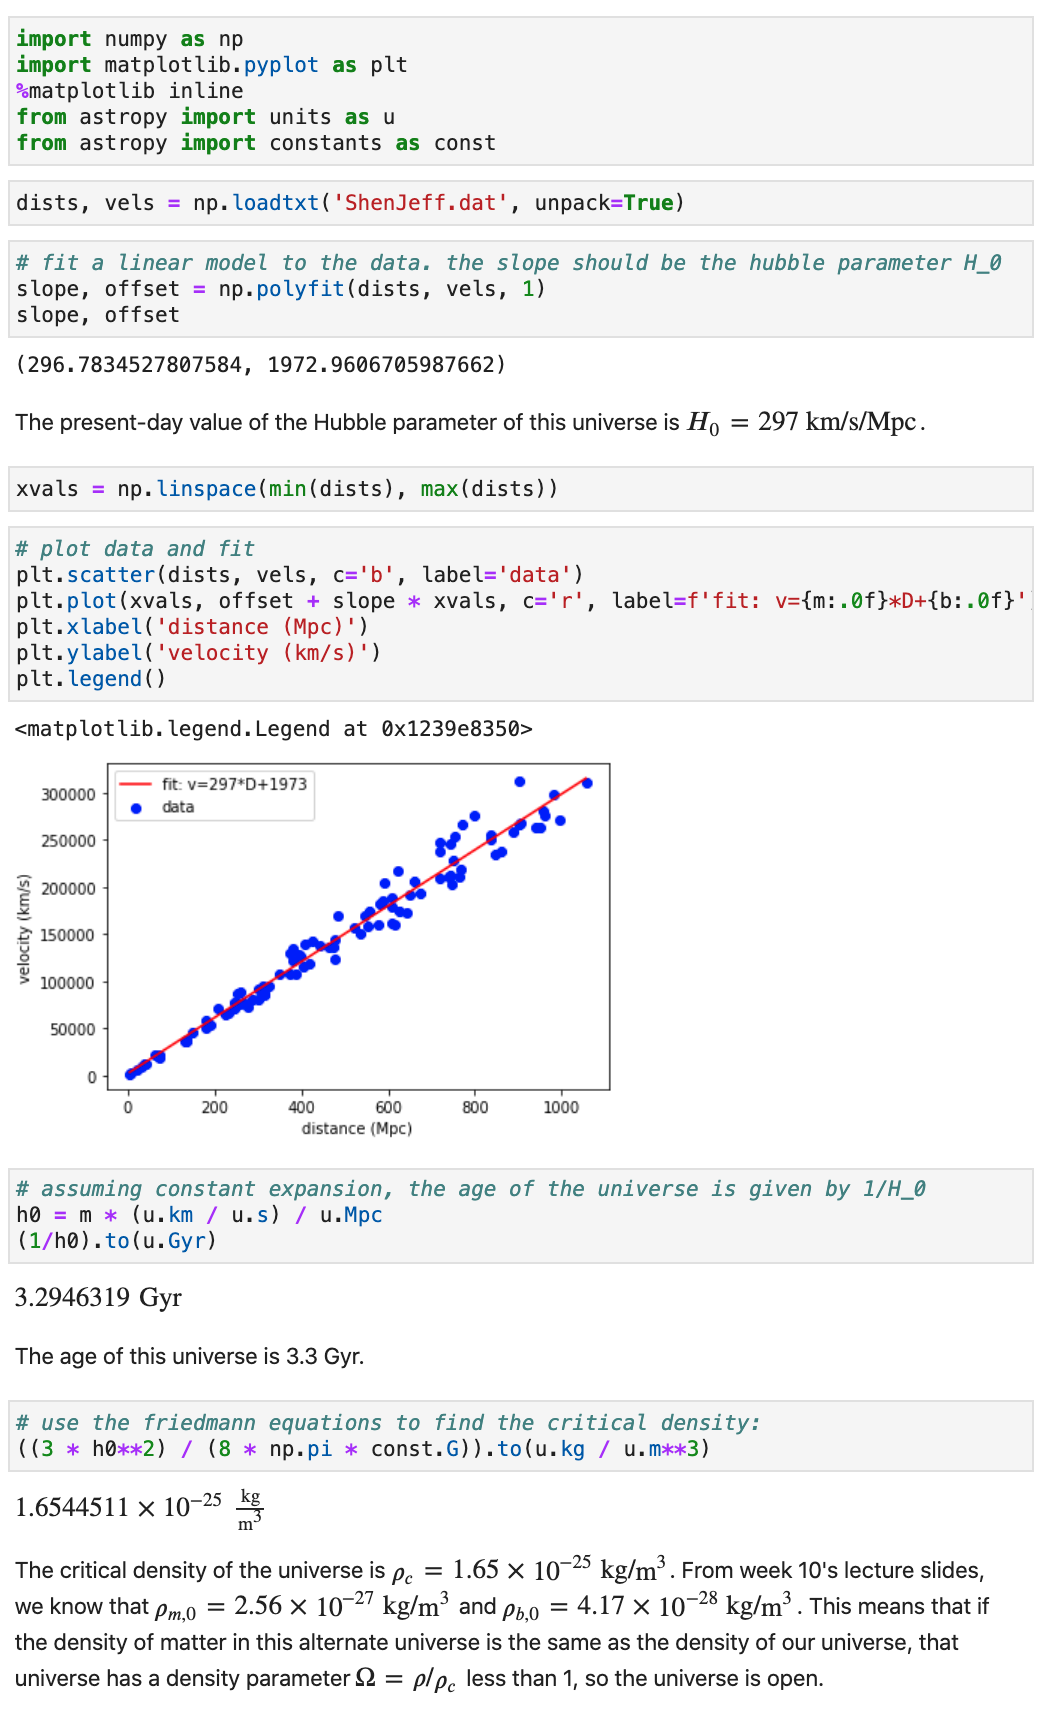
\includegraphics[width=0.78\linewidth]{q5.png}
\end{figure*}

\newpage

\section*{Problem 6}
\begin{enumerate}[label=(\roman*)]
    \item C\&O Eq. 29.10:
        \begin{align*}
            \left[\left(\frac{1}{R}\frac{dR}{dt}\right)^2 - \frac{8}{3}\pi G\rho\right]R^2 = -kc^2.
        \end{align*}
        Multiplying this by $R$, we get 
        \begin{align*}
            \left(\frac{dR}{dt}\right)^2 R - \frac{8}{3}\pi G\rho R^3 = -kc^2R 
        \end{align*}
        Taking the time derivative and applying the product and chain rules to the first term, we get 
        \begin{align*}
            2\frac{dR}{dt}\frac{d^2R}{dt}R + \left(\frac{dR}{dt}\right)^3 - \frac{8}{3}\pi G \frac{d}{dt}(\rho R^3) = \frac{d}{dt}(-kc^2R).
        \end{align*}
        We use C\&O Eq. 29.50 to replace the third term on the left side, then expand the derivative using the chain rule and cancel out a $dR/dt$ term:
        \begin{alignat*}{2}
            &&2\frac{dR}{dt}\frac{d^2R}{dt^2}R + \left(\frac{dR}{dt}\right)^3 + \frac{8}{3}\pi G\frac{P}{c^2}\frac{d(R^3)}{dt} &= -kc^2\frac{dR}{dt} \\
            \implies&&2\frac{dR}{dt}\frac{d^2R}{dt^2}R + \left(\frac{dR}{dt}\right)^3 + \frac{8}{3}\pi G\frac{P}{c^2}3R^2\frac{dR}{dt} &= -kc^2\frac{dR}{dt} \\
            \implies&&2\frac{d^2R}{dt^2}R + \left(\frac{dR}{dt}\right)^2 + 8\pi G\frac{P}{c^2}R^2 &= -kc^2.
        \end{alignat*}
        We can use Eq. 29.10 again to replace the $-kc^2$ term on the right side: 
        \begin{align*}
            2\frac{d^2R}{dt^2}R + \left(\frac{dR}{dt}\right)^2 + 8\pi G\frac{P}{c^2}R^2 &= \left(\frac{dR}{dt}\right)^2 - \frac{8}{3}\pi G\rho R^2.
        \end{align*}
        Cancelling terms and rearranging, we get 
        \begin{align*}
            2\frac{d^2R}{dt^2}R = -8\pi GR^2(\frac{\rho}{3} + \frac{P}{c^2}).
        \end{align*}
        Dividing both sides by $2R$ and then factoring out $1/3$ from the right side, we arrive at C\&O Eq. 29.51:
        \begin{align*}
            \frac{d^2R}{dt^2} = -\frac{4}{3}GR(\rho + \frac{3P}{c^2}).
        \end{align*}
    \item 
    \item 
\end{enumerate}



\end{document}
